
\chapter{Nonlocal Heat Transport and Improved Target Design for X-ray Heating Studies at X-ray Free Electron Lasers}
\label{chap:hef_chapter}

Oliver Hoidn and Gerald T. Seidler\textsuperscript{(*)}

Physics Department, University of Washington, Seattle WA

(*) seidler@uw.edu

The extremely high power densities and short durations of single pulses
of x-ray free electron lasers (XFELs) have opened new opportunities in
atomic physics, where complex excitation-relaxation chains allow for
high ionization states in atomic and molecular systems, and in dense
plasma physics, where XFEL heating of solid-density targets can create
unique dense states of matter having temperatures on the order of the
Fermi energy. We focus here on the latter phenomena, with special
emphasis on the problem of optimum target design to achieve high x-ray
heating into the warm dense matter (WDM) state. We report fully
three-dimensional simulations of the incident x-ray pulse and the
resulting multielectron relaxation cascade to model the spatial energy
density deposition in multicomponent targets, with particular focus on
the effects of nonlocal heat transport due to the motion of high energy
photoelectrons and Auger electrons. We find that nanoscale high-Z/low-Z
multicomponent targets can give much improved energy density deposition
in lower-Z materials, with enhancements reaching a factor of 100. This
has three important benefits. First, it greatly enlarges the
thermodynamic parameter space in XFEL x-ray heating studies of lower-Z
materials. Second, it allows the use of higher probe photon energies,
enabling higher-information content X-ray diffraction (XRD) measurements
such as in two-color XFEL operations. Third, while this is merely one
step toward optimization of x-ray heating target design, the
demonstration of the importance of nonlocal heat transport establishes
important common ground between XFEL-based x-ray heating studies and
more traditional laser plasma methods.

Submitted April 2017 Physical Review B

\section{I. Introduction}

Dense matter under extreme conditions of pressure (P), temperature (T),
or both, is a topic of classic and growing interest across multiple
subfields of contemporary science. \cite{DRAKE2006HIGH, KRISHNAN1998STRUCTURE, FORTNEY2009FRONTIERS, GLENZER2009X, NATIONAL2003HIGH} We focus here on the very
specific case of femtosecond-scale x-ray heating of crystalline matter,
in which there is growing evidence that the lattice often has limited
opportunity to structurally relax during the incident x-ray pulses
{[}6-8{]} and that the loss of crystallinity during the x-ray pulse may
have only modest scientific impact. \cite{CALEMAN2015ULTRAFAST} Such studies hold a
significant and, we propose, unique position for discovery, because they
encompass the case in which the consequences that traditional condensed
phase electronic structure theory has on the structure of
partially-ionized plasmas will be strongest and most easily
interrogated. Hence, the study of crystalline matter at ambient density
but highly elevated electronic temperature holds high potential for
directly testing foundational issues in finite-T density functional
theory, especially including the proper treatment of T-dependent
functionals. \cite{KARASIEV2012GENERALIZED, KARASIEV2012COMPARISON, VALENZA2016WARM}

This point has recently been made by Valenza and Seidler \cite{VALENZA2016WARM}, who
demonstrated that finite-T DFT makes strong, initially counter-intuitive
predictions about the evolution of the absolute and relative Bragg peak
intensities in x-ray diffraction (XRD) from crystalline matter as a
function of electronic temperature on the 1 -- 50 eV scale. The key
point is that XRD provides a more detailed interrogation of the
population of electronic states for crystalline matter than it does for
the more amorphous states interrogated after, e.g., laser shock heating.
Furthermore, it is this temperature dependence that is a key
\emph{microscopic} \emph{observable} of all finite-T DFT approaches: the
central quantity calculated in DFT is, after all, the spatial
distribution of electron density. Therefore, careful characterization of
the real-space charge density at elevated electronic temperatures in a
cool lattice gives a direct path to evaluating different DFT
implementations. This is particularly significant as regards the
temperature-dependent exchange functional, which is essential to
predictions of bulk thermodynamic and elastic properties \cite{KARASIEV2012GENERALIZED, KARASIEV2012COMPARISON, BREDOW2000EFFECT}.

However, in such a research program there is a confounding detail. The
most effective heating by x-rays will occur with lower-energy photons
(that are more strongly absorbed) whereas any detailed interrogation of
the real-space charge distribution by XRD requires the use of higher
energy x-rays to obtain information over a wide momentum transfer range.
{[}12{]} This dilemma raises a question that is new in the XFEL
community but old in the broader plasma physics community: \emph{Given
the incident pulse characteristics and the desired sample material, how
does one design a target to achieve optimal energy density deposition}?

The most comprehensive treatment of this question would include a fully
spatio-temporal treatment of radiative transport as well as electronic
dynamics and electron-atom interactions wherein, again because of the
short time scales, lattice relaxation can be ignored or at least is
secondary. Within this framework, the temporal evolution of
electron-electron and electron-atom interaction includes several stages.
First, the atomic physics of the core levels gives rise to an initial
population of high-energy Auger electrons and photoelectrons that decay
into low-energy (\textless{} 50 eV) electronic excitations (both
collective and single-particle) on the scale of a few femtoseconds. The
resulting collective excitations decay by generating electron-hole pairs
on the time scale of tens of femtoseconds. Subsequent electron-electron
thermalization occurs on the scale of 100 fs -- 1 ps for ambient matter
{[}14-17{]}, but in general has a strong eV-scale temperature
dependence, thus requiring a self-consistent treatment at high incident
flux levels.\cite{FAURE2013DIRECT}

Here, we take a simpler approach with the goal of identifying and
illustrating the most important contributors to x-ray heating and how
their spatial extent strongly influences optimum x-ray heating target
design, in the limited sense of optimizing the deposited net energy
density in the desired sample phase. Specifically, we address the key
questions surrounding nonlocal energy transport by hot electrons. This
topic has a long history in plasma physics, especially for inertial
confinement fusion target design, but enters here with typically
lower-energy electrons, i.e., keV-scale, than are important in ICF and
in direct-drive laser-heating studies. This causes the energy deposition
length of the hot electrons to decrease from the 100-1000 µm scale for
MeV electrons in laser experiments to instead only
$\sim$50-200 nm, depending on the atomic number of the
species present in the XFEL x-ray heating target.

It is this much shorter length scale that brings us to consider
multicomponent nanoscale targets for x-ray heating so that the influence
of nonlocal energy transport by the hot electrons can be usefully
engineered. While the importance of nanoscale energy transport has not
previously been discussed in the context of XFEL heating target design,
it has been studied and exploited in other experimental contexts. For
example, there exists a significant body of literature in the medical
physics community concerned with using gold nanoparticles for dose
enhancement in radiotherapy treatment. \cite{LEE2012GEOMETRY, LEUNG2011IRRADIATION} A contrasting
application of nonlocal energy transport is found in the macromolecular
crystallography community, where there is interest in the use of
submicron incident x-ray beams so that a large fraction of high-energy
electrons escape the beam spot before slowing down, thus reducing
radiation damage in the probed sample volume. \cite{STERN2009REDUCING, FINFROCK2013MITIGATION, FINFROCK2010SPATIAL, NAVE2005TOWARDS, SANISHVILI2011RADIATION}

With the above context established, we consider here a nanostructured
target design that enhances energy deposition in a sample material using
nonlocal heat transport from a more strongly x-ray absorbing material in
contact with the sample -- we refer to this second material as a
`cladding' as a matter of convenience, for closer contact to the
terminology of laser-shock target design, even when the geometry may not
strictly be cladded. Fig. \ref{fig:hef_image1} sketches several corresponding geometries,
but in the current paper we concentrate on the particularly simple one
of Fig. \ref{fig:hef_image1} (c), consisting of a single thin film of sample material clad
with Au. We use the Monte Carlo code PENELOPE to simulate
three-dimensional electron-photon transport and the corresponding
spatial distributions of deposited energy to demonstrate two benefits to
the design: first, it significantly enhances in-sample energy
deposition, and second, it relaxes constraints on XFEL pump photon
energy in a way that substantially increases the information content of
XRD measurements in certain experimental contexts.

We proceed as follows. In section II, we describe the methods used to
simulate photoionization and electron transport in a nanostructured
target and discuss the simplifying approximations on which we rely. In
section III, we present and discuss simulation results of multilayer
targets consisting of sample material clad on one or two sides with
gold. We find that such a cladding configuration significantly increases
deposited energy density in a sample material, with the largest
enhancement in low-Z samples. We argue that this enhanced effect in
low-Z samples opens the door to wide-angle x-ray diffraction (wide-angle
XRD), with significant utility for studying the time dynamics of the
energy relaxation cascade for both electronic and lattice/ion degrees of
freedom in such materials. These observations are particularly relevant
in the context of two-color x-ray pump x-ray probe experiments at
XFELs\cite{HOIDN2017NONLOCAL, INOUE2016OBSERVATION, HO2015RESONANCE, ALLARIA2013TWO}, but also serve more generally to establish the
importance of nanoscale nonlocal heat transport in high-intensity XFEL
studies. Finally, in section IV we conclude.

\section{II. Methods}

The simulation of electron transport in condensed matter is an area of
ongoing research. In addition to continuing development of
well-established codes in the high-energy experimental particle physics
community \cite{AGOSTINELLI2003GEANT4}, new developments include incorporation of
\emph{ab initio} band structure calculations in order to accurately
model the electron mean free paths of interband transitions and plasmon
excitations from relativistic energies down to a few eV. \cite{GAO2013MONTE, PRANGE2014RADIATION}

In the regime relevant to the present study, calculation of the spatial
distribution of deposited energy caused by absorption of a hard x ray
requires accurate treatment of the processes that describe scattering of
photo- and Auger electrons at the 100 eV to 10 keV scale (generation of
secondary x-ray photons, though present, plays a negligible role in
energy transport). The simplest atomic treatments of elastic and
inelastic scattering demonstrate that, for mid- and high-Z elements, the
ratio of elastic to inelastic total cross sections is of order unity and
that characteristic elastic scattering angles are sufficiently large
(for instance, of order 1 rad for $\sim$1 keV electrons) to
influence deposited energy distributions. \cite{POLLOCK2017ACCURACY} Both components,
therefore, must receive accurate treatments to adequately model spatial
energy deposition distributions in a nanostructured target.

The spatial distribution of deposited energy is determined by the
electron stopping power \(\frac{\text{dE}}{\text{dz}}\), which in a
classical treatment is related to a material's dielectric function
\(\varepsilon(q,\ \ \omega)\) by

\begin{quote}
\(\frac{\text{dE}}{\text{dz}} = \ \frac{2^{2}}{\pi a_{0}m_{0}v^{2}}\ \iint_{}^{}\frac{q_{y}\omega\ Im\lbrack\frac{- 1}{\varepsilon(q,\ \ \omega)\rbrack}}{{q_{y}}^{2} + \left( \frac{\omega}{v} \right)^{2}}dq_{y}d\omega,\)
(1)
\end{quote}

where ω is angular frequency, \(q\) is momentum transfer (with \(q_{y}\)
the magnitude of the component for momentum transfer perpendicular to
the z-direction), \(a_{0}\) is the Bohr radius, \(m_{0}\) is the
electron mass, and \(v\) is the electron velocity. \cite{POLLOCK2017ACCURACY} In the case
of electron showers generated by 5-10 keV photons, the electron stopping
power's dependence on \(v\) causes nonlocal energy transport to be
dominated by the highest-energy Auger and photoelectrons. Though the
slower time evolution of the subsequent electronic and lattice dynamics
may be neglected in the present context of simulating fsec-scale energy
transport, the possibility of interrogating it by time-resolved XFEL
pump-probe measurement is an interesting topic in its own
right.\cite{HOIDN2017NONLOCAL}

To model the above physics we used the code PENELOPE, which implements
particle-tracking Monte Carlo simulations of electron showers generated
by x-ray photoionization. PENELOPE uses total and differential
cross sections based on several physical models. Briefly, it derives
elastic and inner-shell inelastic cross sections from strictly atomic
wave functions, while the valence contribution to the inelastic double
differential cross section is based on the Born approximation and
generalized oscillator strength model of Liljequist \cite{LILJEQUIST1983SIMPLE}, with an
energy loss-dependent normalization that allows the model to replicate
empirical stopping power data (provided as program input). Although the
inelastic scattering cross section is dominated by low-energy loss
collisions, inner shells contribute the majority of the stopping power
for several-keV electrons, which account for the longest-range energy
transport. For electrons of those energies the stopping power of a
compound may be approximated within five percent by a stoichiometric sum
based on atomic treatments of its constituents (an observation referred
to as Bragg's rule). \cite{ZEISS1977ACCURATE} Consequently we employed material data
files generated by the PENELOPE 2011 program MATERIAL, which applies
this approximation to infer stopping powers of arbitrary compounds using
data from the NIST ESTAR database. \cite{BERGER1995ESTAR}

\section{III. Results and discussion}

We now present results for several realizations of our nanostructured
target design, all of which consist of thin films clad with Au on one or
both sides. The heating of an Fe thin film via nonlocal heat transport
by hot electrons is illustrated in Fig. \ref{fig:hef_image2}, which shows a two-dimensional
projection of electron trajectory traces in an Au-Fe-Au trilayer
stimulated with 7 keV incident photons. The color-coding of the tracks
shows that, due to the much larger number of photoexcitations in the Au
cladding compared to Fe inclusion, most hot electrons propagating in the
Fe are part of a photoionization relaxation cascade originating in the
cladding. Inelastic scattering of these hot electrons is the dominant
contribution to energy deposition in the central Fe region, as
quantified by Fig. \ref{fig:hef_image3}, which compares the linear energy deposition of
several Au-Fe-Au trilayer configurations to that in bare Fe.

Photoionization by 7 keV photons yields mean energy deposition lengths
\(l\) of 15.0 nm and 35.3 nm, respectively, in simulated bare Fe and
bare Au targets, where
\(l = \ \int_{z = 0}^{\infty}{z(\overrightarrow{r})\ \rho\left( \overrightarrow{r} \right)\ d^{3}\overrightarrow{r}}\),
with \(\rho\left( \overrightarrow{r} \right)\) the volume density of
deposited energy and \(z\) the magnitude of the projection of
\(\overrightarrow{r}\) onto a fixed, arbitrary unit vector. Consistent
with the above characteristic lengths, we found that absorbed energy
density in the Fe inclusion saturates beyond an Au cladding thickness of
50 nm. Fig. \ref{fig:hef_image3} (a) shows the deposited energy distribution in a bare
Fe\textsubscript{3}O\textsubscript{4} target and in several Au-
Fe\textsubscript{3}O\textsubscript{4}-Au trilayers with varying
thicknesses of the Fe\textsubscript{3}O\textsubscript{4} inclusion. An
interior layer thickness of 50 nm results in a factor of five
enhancement in deposited energy density relative to the bare
Fe\textsubscript{3}O\textsubscript{4} target. The increase in deposited
energy density in a clad sample compared to a bare one is significantly
larger for lower-Z materials, reaching a factor of 100 for an Au-C-Au
target of the same geometry (Fig. \ref{fig:hef_image4}).

These enhancements in energy deposition increase the accessible
thermodynamic parameter space in all XFEL heating experiments, which is
particularly significant for experimental diagnostics that require
deviation from optimal pump pulse characteristics and are therefore
normally incompatible with heating studies, for instance XRD. We
illustrate this in Fig. \ref{fig:hef_image5}, which compares the energy deposition in
Au-Fe-Au and Au-Fe\textsubscript{3}O\textsubscript{4}-Au targets
stimulated with photons below the \emph{K}-edge of Fe to that in a bare
Fe target heated by photons above the edge. Nonlocal heating of the
former samples compensates for the reduction in sample heating caused by
lowering the incident photon energy below the Fe \emph{K}-edge; the
multicomponent targets thus allow improving the ratio of signal to
(fluorescence) background while---in the more favorable case of
Fe\textsubscript{3}O\textsubscript{4}--maintaining an energy deposition
density comparable to the highest level possible with an equivalent
monolithic target. However, Fig. \ref{fig:hef_image6} also demonstrates a tradeoff of the
cladding's presence: the diffracted signal from Au is stronger than that
from the sample, making the described reduction in background worthwhile
only assuming sufficient separation between Bragg peaks of the sample
and cladding.

Low-Z sample materials provide a separate, independently interesting,
case for the use of structured target design in XRD studies. In such
materials, nonlocal heat transport is effective over a much wider range
of incident photon energies compared to direct x-ray absorption. Until
now, x-ray heating studies of low-Z materials, such as graphite, have
required incident photon energies below 3 keV to reach HED conditions
(\textgreater{} $\sim$1 eV temperatures) due to these
materials' small photoelectric cross sections in the hard X ray (photon
energy \textgreater{} 5 keV) regime. This restriction limits the
kinematically accessible range of momentum transfers in XRD, which
correspondingly reduces available information on real-space charge
density.

This creates an experimental dilemma with scientific consequences. For
example, Hau-Riege et al.\cite{HAU2012ULTRAFAST} showed evidence for ultrafast melting
of graphite during a 40 fs-long XFEL pulse but were limited, for the
reason described above, to using 2 keV incident photons, yielding
diffraction from only the 002 Bragg reflection of graphite. The authors
interpreted quenching upon heating of the 002 peak as evidence of
nonthermal lattice melting. However, Valenza \emph{et al.}\cite{VALENZA2016WARM}
questioned this conclusion based on simulated diffraction using
frozen-core finite-T DFT calculations, which predicted strong quenching
of the graphite 002 reflection due to purely electronic reorganization
in crystalline graphite at 10 eV electronic temperature. In graphite and
other low-Z systems, the only means of unambiguously separating lattice
disorder from electronic heating in the XRD signal is to probe several
Bragg peaks, including the lowest-order reflections and their harmonics.
{[}12{]}

It is therefore interesting to ask whether high energy-densities can be
achieved in graphite when using photons suitable for wide-angle
scattering. In Fig. \ref{fig:hef_image4} we show the deposited energy densities in Au-C-Au
trilayers of several interior thicknesses, once again using 7 keV
incident photons (sufficient to probe the 006 reflection of graphite).
The deposited energy density in the interior layer is at least a factor
of 100 greater compared to an unclad sample with the same incident
photon energy, and a factor of two greater compared to an unclad sample
stimulated with 2 keV photons. Indirect heating via high-Z cladding thus
eliminates the constraint of selecting incident photon energies near a
low-Z material's small core binding energies, making wide-angle XRD
possible. In the context of carbon, the weakness of the XRD from C
compared to Au can be uniquely compensated with a highly-oriented
pyrolytic graphite (HOPG) sample, whose high-reflectivity 00\emph{l}
peaks yield much higher signal to background ratios than the powder-like
Bragg and thermal diffuse scattering of polycrystalline Au. Similar
configurations exploiting mosaic or single-crystal samples may enhance
wide-angle XRD on a variety of low-Z systems, offering a much-improved
ability to experimentally test predictions of finite-T DFT-based
modeling of electronic structure in low-Z condensed matter, where
finite-T effects are easiest to identify because of the relatively large
valence-electron contribution to the XRD signal.\cite{VALENZA2016WARM}

The simulations presented in this paper constitute a first demonstration
of a particularly simple implementation of structured target design. One
can imagine several improved designs that achieve the same level of
nonlocal sample heating while averting some of the disadvantages of our
multilayer approach. For example, a uniform mixture of small
(\textless{} 50 nm diameter) sample and heater nanoparticles would show
similar mean deposited energy densities to a multilayer target and can
be prepared by, e.g., spin coating or drop-casting. Such targets would
have more homogeneous heating and would additionally allow preparation
of much thicker targets and give much higher scattered intensities. A
similar result may be possible using electrochemical or vapor deposition
to embed sample materials inside porous high-Z metal
substrates.\cite{BAK2014EFFICIENT, BAGGE2014QUANTITATIVE} Two-color XFEL experiments may also lend
themselves to lithographically patterned designs with concentric
cylindrical volumes of (inner) sample and (outer) cladding materials,
wherein the more tightly-focused probe pulse would be inscribed in a
volume free of cladding material. Such a configuration would have the
intention of reducing (cladding) background relative to signal, which
would be particularly useful for weakly-diffracting low-Z samples.

\section{IV. Conclusion}

We model the spatial distribution of deposited energy in nanostructured
targets for hard x-ray XFEL heating experiments using the Monte Carlo
code PENELOPE. We find that two-component targets consisting of a sample
material and high-Z cladding achieve substantial nonlocal heating of the
sample via the relaxation cascade following transport of multi-keV Auger
and photoelectrons. We argue that this target design approach will bring
substantial benefits to XFEL heating experiments in the following ways:
first, by enlarging their accessible thermodynamic parameter space and
second, by improving the capability of x-ray diffraction diagnostics to
characterize finite-temperature electronic structure and to distinguish
between thermalization of the electronic and lattice degrees of freedom
in crystalline warm dense matter systems.

\subsection{Acknowledgements}

We thank Joshua Kas for useful discussions. This work was supported by
the United States Department of Energy, Basic Energy Sciences, under
grant DE-SC00008580 and by the Joint Plasma Physics Program of the
National Science Foundation and the Department of Energy under grant
DE-SC0016251. \textbf{\\References}

{[}1{]} R. P. Drake, \emph{High-Energy-Density Physics: Fundamentals,
Inertial Fusion, and Experimental Astrophysics} (Springer, 2006), Shock
Wave and High Pressure Phenomena.

{[}2{]} S. Krishnan, S. Ansell, J. J. Felten, K. J. Volin, and D. L.
Price, Physical Review Letters \textbf{81}, 586 (1998).

{[}3{]} J. J. Fortney, S. H. Glenzer, M. Koenig, B. Militzer, D. Saumon,
and D. Valencia, Physics of Plasmas \textbf{16}, 041003 (2009).

{[}4{]} S. Glenzer and R. Redmer, Review of Modern Physics \textbf{81},
1625 (2009).

{[}5{]} R. C. Davidson, National Research Council of the National
Academies\emph{,} \emph{Frontiers in High Energy Density Physics: The
X-Games of Contemporary Science} 2003.

{[}6{]} S. P. Hau-Riege, Physical Review E \textbf{87}, 4, 053102
(2013).

{[}7{]} S. Boutet \emph{et al.}, Science \textbf{337}, 362 (2012).

{[}8{]} H. N. Chapman \emph{et al.}, Nature \textbf{470}, 73 (2011).

{[}9{]} C. Caleman, N. Timneanu, A. V. Martin, H. O. Jonsson, A. Aquila,
A. Barty, H. A. Scott, T. A. White, and H. N. Chapman, Optics Express
\textbf{23}, 1213 (2015).

{[}10{]} V. V. Karasiev, T. Sjostrom, and S. B. Trickey, Physical Review
B \textbf{86}, 115101 (2012).

{[}11{]} V. V. Karasiev, T. Sjostrom, and S. B. Trickey, Physical Review
E \textbf{86}, 056704 (2012).

{[}12{]} R. A. Valenza and G. T. Seidler, Physical Review B \textbf{93},
115135 (2016).

{[}13{]} T. Bredow and A. R. Gerson, Physical Review B \textbf{61}, 5194
(2000).

{[}14{]} W. S. Fann, R. Storz, H. W. K. Tom, and J. Bokor, Physical
Review B \textbf{46}, 13592 (1992).

{[}15{]} J. Faure \emph{et al.}, Physical Review B \textbf{88}, 075120
(2013).

{[}16{]} M. Lisowski, P. A. Loukakos, U. Bovensiepen, J. Stähler, C.
Gahl, and M. Wolf, Applied Physics A \textbf{78}, 165 (2004).

{[}17{]} I. Timrov, T. Kampfrath, J. Faure, N. Vast, C. R. Ast, C.
Frischkorn, M. Wolf, P. Gava, and L. Perfetti, Physical Review B
\textbf{85}, 155139 (2012).

{[}18{]} C. Lee, N. N. Cheng, R. A. Davidson, and T. Guo, The Journal of
Physical Chemistry C \textbf{116}, 11292 (2012).

{[}19{]} M. K. K. Leung, J. C. L. Chow, B. D. Chithrani, M. J. G. Lee,
B. Oms, and D. A. Jaffray, Medical Physics \textbf{38}, 624 (2011).

{[}20{]} E. A. Stern, Y. Yacoby, G. T. Seidler, K. P. Nagle, M. P.
Prange, A. P. Sorini, J. J. Rehr, and A. Joachimiak, Acta
Crystallographica Section D-Biological Crystallography \textbf{65}, 366
(2009).

{[}21{]} Y. Z. Finfrock, E. A. Stern, R. W. Alkire, J. J. Kas, K.
Evans-Lutterodt, A. Stein, N. Duke, K. Lazarski, and A. Joachimiak, Acta
Crystallographica Section D-Biological Crystallography \textbf{69}, 1463
(2013).

{[}22{]} Y. Z. Finfrock, E. A. Stern, Y. Yacoby, R. W. Alkire, K.
Evans-Lutterodt, A. Stein, A. F. Isakovic, J. J. Kas, and A. Joachimiak,
Acta Crystallographica Section D-Biological Crystallography \textbf{66},
1287 (2010).

{[}23{]} C. Nave and M. A. Hill, Journal of Synchrotron Radiation
\textbf{12}, 299 (2005).

{[}24{]} R. Sanishvili \emph{et al.}, Proceedings of the National
Academy of Sciences of the United States of America \textbf{108}, 6127
(2011).

{[}25{]} A. A. Lutman, R. Coffee, Y. Ding, Z. Huang, J. Krzywinski, T.
Maxwell, M. Messerschmidt, and H. D. Nuhn, Physical Review Letters
\textbf{110}, 134801, 134801 (2013).

{[}26{]} A. Marinelli, A. A. Lutman, J. Wu, Y. Ding, J. Krzywinski, H.
D. Nuhn, Y. Feng, R. N. Coffee, and C. Pellegrini, Physical Review
Letters \textbf{111}, 134801, 134801 (2013).

{[}27{]} I. Inoue \emph{et al.}, Proceedings of the National Academy of
Sciences \textbf{113}, 1492 (2016).

{[}28{]} P. J. Ho, E. Kanter, and L. Young, Physical Review A
\textbf{92}, 063430 (2015).

{[}29{]} E. Allaria \emph{et al.}, Nature Communications \textbf{4},
2476 (2013).

{[}30{]} S. Agostinelli \emph{et al.}, Nuclear Instruments and Methods
in Physics Research Section A: Accelerators, Spectrometers, Detectors
and Associated Equipment \textbf{506}, 250 (2003).

{[}31{]} F. Salvat, J. M. Fernández-Varea, and J. Sempau,
\emph{PENELOPE-2006: A code system for Monte Carlo simulation of
electron and photon transport} (OECD Publishing, Paris, 2006).

{[}32{]} F. Gao, Y. Xie, Z. G. Wang, S. Kerisit, D. X. Wu, L. W.
Campbell, R. M. Van Ginhoven, and M. Prange, Journal of Applied Physics
\textbf{114}, 173512 (2013).

{[}33{]} M. Prange, D. Wu, Y. Xie, L. W. Campbell, F. Gao, and S.
Kerisit, \emph{Radiation response of inorganic scintillators: insights
from Monte Carlo simulations} (SPIE, 2014), 92130L.

{[}34{]} R. F. Egerton, \emph{Electron energy-loss spectroscopy in the
electron microscope} (Springer Science \& Business Media, 2011).

{[}35{]} J. M. Fernández-Varea, R. Mayol, D. Liljequist, and F. Salvat,
Journal of Physics: Condensed Matter \textbf{5}, 3593 (1993).

{[}36{]} D. Liljequist, Journal of Physics D: Applied Physics
\textbf{16}, 1567 (1983).

{[}37{]} G. D. Zeiss, W. J. Meath, J. C. F. MacDonald, and D. J. Dawson,
Radiation Research \textbf{70}, 284 (1977).

{[}38{]} M. J. Berger, NIST\emph{,} \emph{ESTAR, PSTAR, and ASTAR:
Computer programs for calculating stopping-power and range tables for
electrons, protons, and helium ions}, 1992.

{[}39{]} S. P. Hau-Riege \emph{et al.}, Physical Review Letters
\textbf{108}, 217402 (2012).

{[}40{]} C. H. Bak, K. Kim, K. Jung, J.-B. Kim, and J.-H. Jang, Journal
of Materials Chemistry A \textbf{2}, 17249 (2014).

{[}41{]} M. Bagge-Hansen \emph{et al.}, The Journal of Physical
Chemistry C \textbf{118}, 4078 (2014).

\begin{figure}[h]
\caption{
Representations of three types of multicomponent
targets composed of sample material (green) and heater cladding
(yellow). (a): A porous subtrate filled with sample material; (b): a
mixture of cladding and sample nanoparticles embedded in a solid matrix;
(c): a multilayer film.
}
\label{fig:hef_image1}
\centering
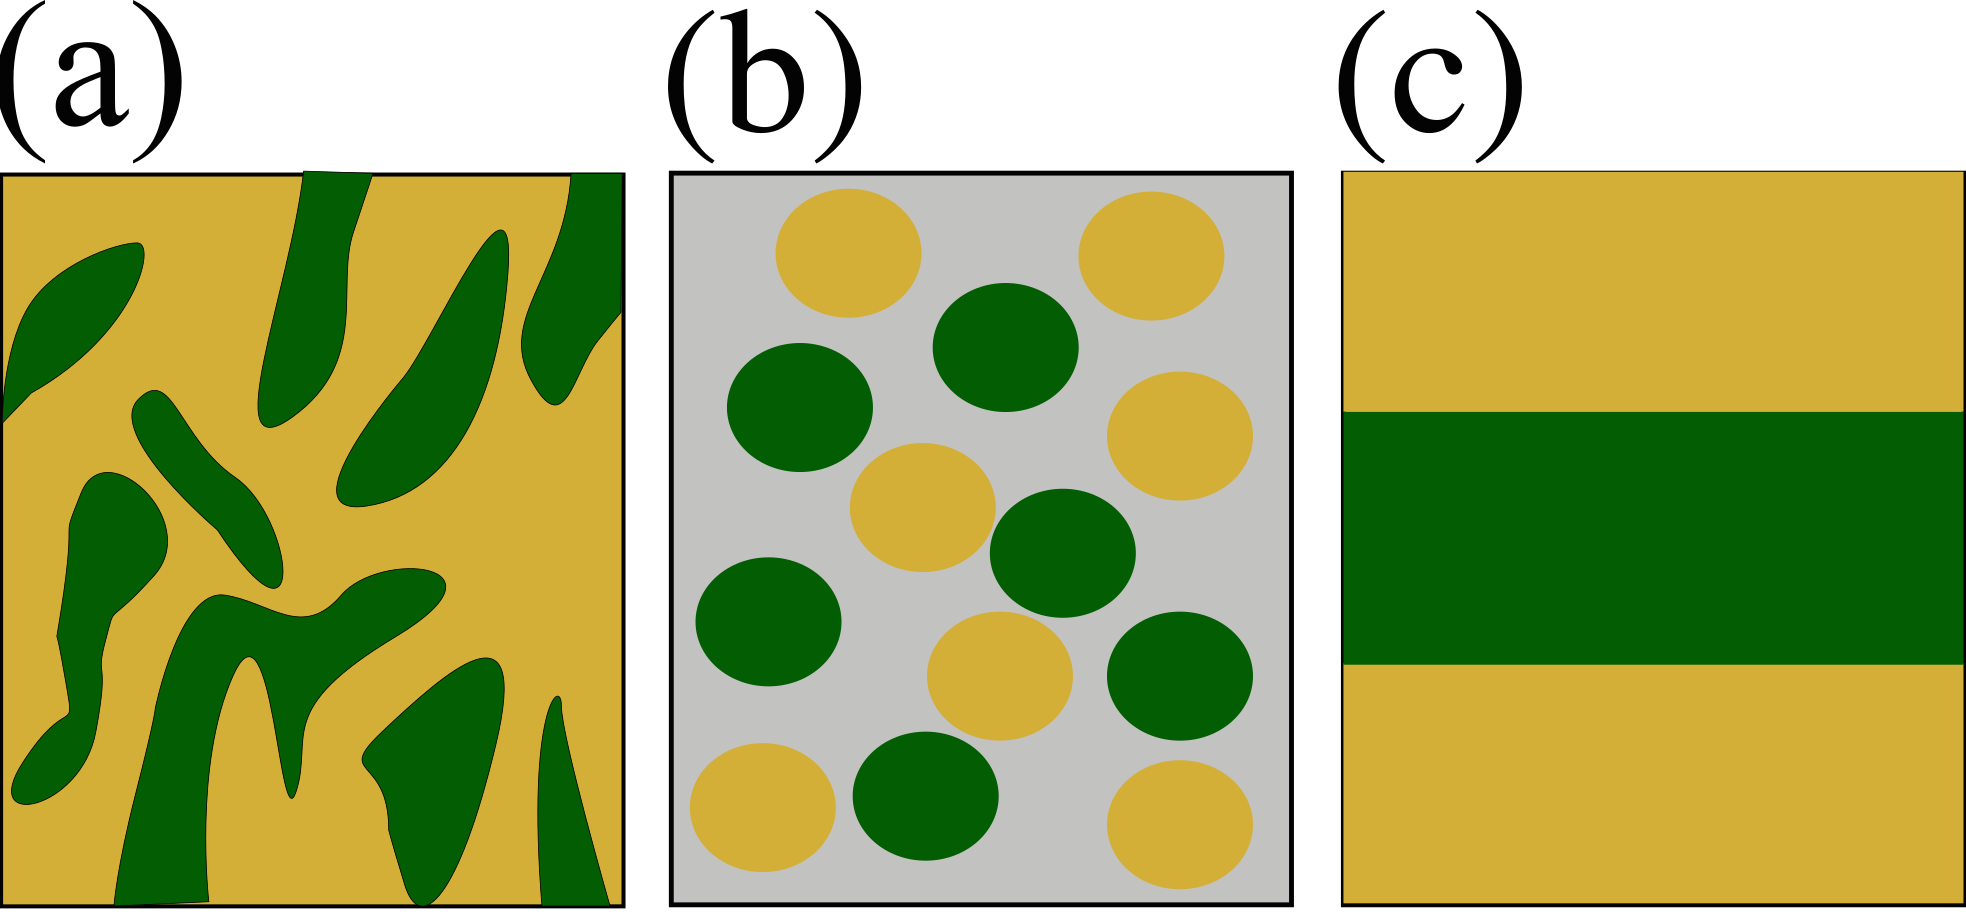
\includegraphics[scale=0.2]{hef/image1.png}
\end{figure}

\begin{figure}[h]
\caption{
Visualization of a 3-D Monte Carlo simulation of
electron transport in an Au-Fe-Au target heated by 7 keV photons,
incident normally from the top of the page. Electron tracks are
projected onto the plane of the page; showers resulting from
photoexcitation of Au and Fe atoms are red and blue, respectively. Note
that most of the electron tracks in the Fe are due to absorption events
in the Au.
}
\label{fig:hef_image2}
\centering
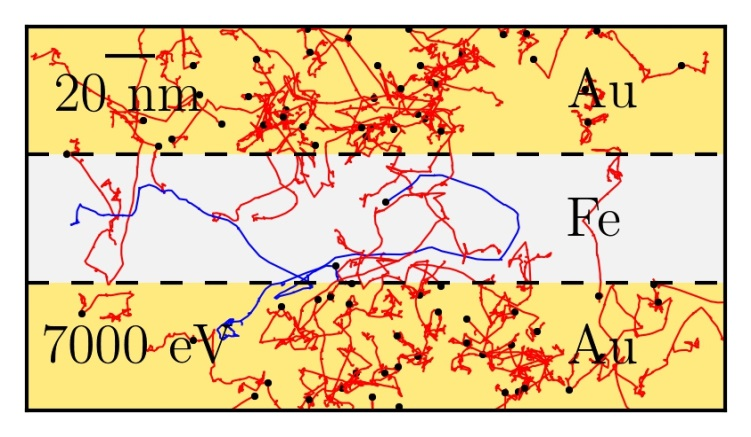
\includegraphics[scale=1.0]{hef/image2.jpeg}
\end{figure}

\begin{figure}[h]
\caption{
(a) Linear energy deposition density generated by 7 keV
photons incident on an Au-Fe\textsubscript{3}O\textsubscript{4}-Au
target, displayed for several thicknesses of the central
Fe\textsubscript{3}O\textsubscript{4} layer and a fixed Au cladding
thickness of 50nm. (b) Histograms of energy deposition density in volume
elements of the Fe\textsubscript{3}O\textsubscript{4} inclusions in
Au-Fe\textsubscript{3}O\textsubscript{4}-Au targets, displayed for
several thicknesses of the Au cladding and a fixed
Fe\textsubscript{3}O\textsubscript{4} layer thickness of 50 nm.
}
\label{fig:hef_image3}
\centering
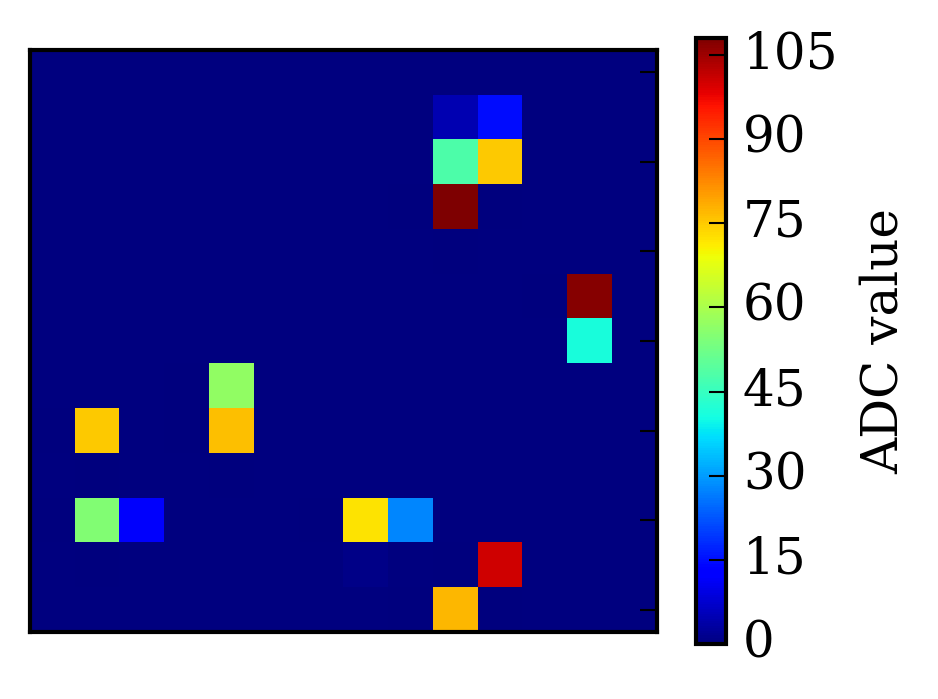
\includegraphics[scale=0.3]{hef/image3.png}
\end{figure}


\begin{figure}[h]
\caption{
%\hyperdef{}{OLEux5fLINK3}{}{\hyperdef{}{OLEux5fLINK4}{}{\hyperdef{}{OLEux5fLINK5}{}{}}}\textbf{4}.
Linear energy deposition due to 7 keV photons incident on an Au-C-Au
target displayed for several thicknesses of the central C layer and a
fixed outer cladding thickness of 50nm.
}
\label{fig:hef_image4}
\centering
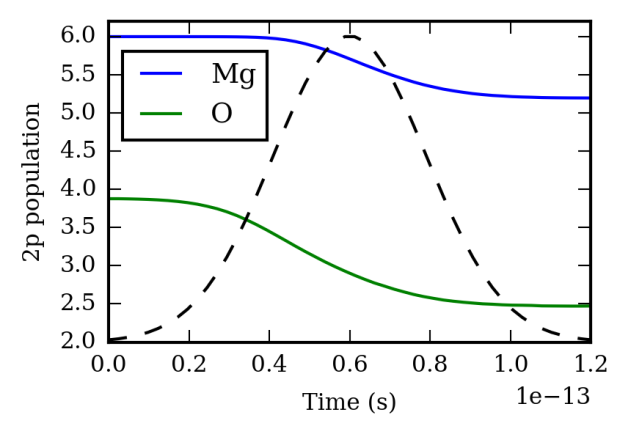
\includegraphics{hef/image4.png}
\end{figure}

\begin{figure}[h]
\caption{
%\hyperdef{}{OLEux5fLINK3}{}{\hyperdef{}{OLEux5fLINK4}{}{\hyperdef{}{OLEux5fLINK5}{}{}}}\textbf{4}.
Linear energy deposition in layered Au-Fe-Au and
Au-Fe\textsubscript{3}O\textsubscript{4}-Au targets of 150 nm total
thickness stimulated by 7 keV photons. Dashed lines indicate energy
deposition in bulk Fe\textsubscript{3}O\textsubscript{4} and Fe at
photon energies of 7.12 keV (above the iron K-edge) and 7 keV (below the
edge). The multilayer configuration sufficiently enhances energy
deposition so as to partially compensate for the difference between pre-
and above-edge x-ray photoelectric cross sections. The benefit is
particularly pronounced in Fe\textsubscript{3}O\textsubscript{4} due to
its much lower density and photoelectric cross-section.
}
\label{fig:hef_image5}
\centering
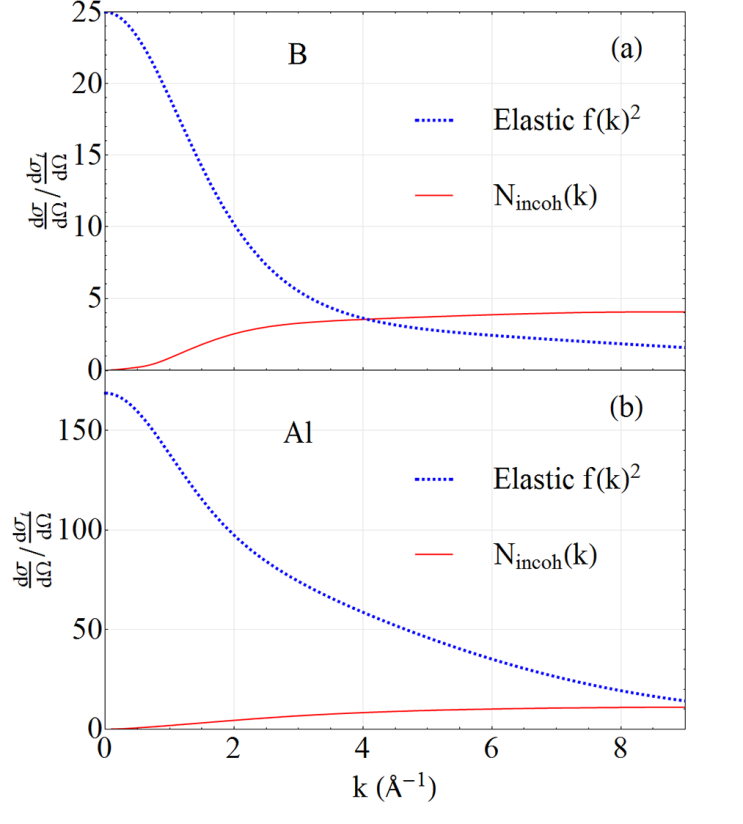
\includegraphics{hef/image5.png}
\end{figure}

\begin{figure}[h]
\caption{
Simulated powder diffraction of 50 nm Au-50 nm
Fe\textsubscript{3}O\textsubscript{4}-50 nm Au stimulated by X-rays
below the Fe K-edge (blue) compared to that resulting from photons above
the edge incident on bare Fe\textsubscript{3}O\textsubscript{4},
including fluorescence background(green).
}
\label{fig:hef_image6}
\centering
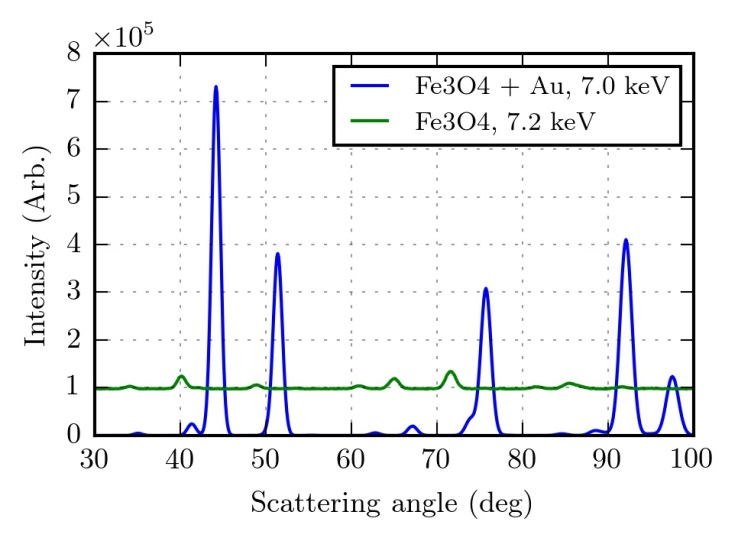
\includegraphics{hef/image6.jpeg}
\end{figure}



